\documentclass[twocolumn,11pt]{asme2ej}

\usepackage{epsfig} %% for loading postscript figures

\title{STAT 154: Project 1 Redwood Data Report}

%%% first author
\author{Jilin Cao, Sizhuo (Cindy) Liu
    \affiliation{
	3033278367, 3032082925
    }	
}

%%% second author
%%% remove the following entry for single author papers
%%% add more entries for additional authors
\author{
    \affiliation{
    }
}

\begin{document}

\maketitle    

\section*{Introduction}

The purpose of this report is to conduct detailed data analysis on datasets from the Redwood Experiment using machine learning and other statistical concepts. 

The paper consists of five major parts: data collection, data cleaning, data exploration, presentation of findings, and graph critiques. In data collection, the background and source of data was explained from deep reading of the research paper. Data cleaning was then carried out in which all irrelevant data or major outliers were removed. Methods such as PCA and linear regression model were then applied to explore the relationships between the major variables. The findings from the data analysis were also summarized. In addition, critiques on the potential improvements of the graphs presented in the research paper were also provided.

%%%%%%%%%%%%%%%%%%%%%%%%%%%%%%%%%%%%%%%%%%%%%%%%%%%%%%%%%%%%%%%%%%%%%%
\section{Data collection}

The research paper presents a case study of a wireless sensor network recorded on a redwood tree, display an overview of the data, and describes the trends and gradients of a large dataset with multidimensional analysis. The purpose of the study was to explore the use of wireless sensor network as a means of peceiving complex interactions due to its capability of producing dense temporal and spatial monitoring of large volumes. The data was collected on a 70-meter redwood tree in Sonoma, California over the course of one summer. Having obtained the results and conducted multidimensional analysis, range analysis, and combined analysis, the author reached the conclusion that the sensor network macroscope implemented in the study did in fact capture the complex environmental dynamics of the microclimate surrounding the redwood tree. Although the amount of data obtained from the successful implementation of the sensor network was very large and extracting information from such a large dataset is difficult, the use of multidimensional analysis has made this data collection problem more tractable. 

A suite of sensors were selected and integrated with the wireless sensor node platform. The sensors were deployed onto the 70-meter redwood tree starting at 15 meters above the ground level. Nodes were distributed evenly along this vertical distance with roughly a 2-meter spacing between each of them. Such a spatial density ensures that enough data would be captured to allow for accurate interpolation in the analysis stage. In terms of angular location, the sensors were all deployed on the west side of the tree as this area has a relatively thicker canopy that provides the most buffering against direct environmental effects. The nodes were placed about 0.1 to 1.0 m from the tree trunk. Such a close distance ensures that the microclimatic trends captured by the sensors would affect the tree directly. 

The entire data collection process lasts one entire month during early summer, as this is the period in which dynamic microclimatic variation is the greatest. Samples of data are collected from the sensors once every 5 minutes as the author believes that this frequency is large enough to collect sufficient data for analysis. 

The main variables of interests were simply the traditional climate variables: temperature, humidity, and light level. For light levels, both incident (direct) and reflected (ambient) levels of photosynthetically active radiation are collected. This is because the incident level provides information about the tree’s energy available for photosynthesis, while the reflected level allows for the validation of satellite remote sensing measurements of land surface reflectance. 

According to the author, a backup is set up in case of network failure and also viewed as a basis for analyzing the performance of the network throughout this case study. Such backup is the local data logging system. The data in sonoma-data-log.csv records the data displayed in this local data logging system while the data in sonoma-data-net.csv is obtained from the wireless network. Data from sonoma-data-log.csv is expected to be more comprehensive as its recordings are not directly affected by the performance of the network level, but only the performance of the sensors. 

%%%%%%%%%%%%%%%%%%%%%%%%%%%%%%%%%%%%%%%%%%%%%%%%%%%%%%%%%%%%%%%%%%%%%%
\section{Data cleaning}
\subsection{Check Variable Consistency Between Datasets}

At the start of the data cleaning process, the differences and similiarities between the data obtained from the local data log and the wireless network were observed by plotting histograms of each variable and comparing them side by side. The plots indicate that the majority of the variables have completely different distributions depending on the dataset from which they were obtained. For example, the graph Fig.1. indicates the humidity data from both data sets and the histograms indicate that they clearly follow completely different distributions. This is the case for most of the variables except for \textbf{hamatop}  and \textbf{hamabot}.  

\begin{figure}
    \centering
    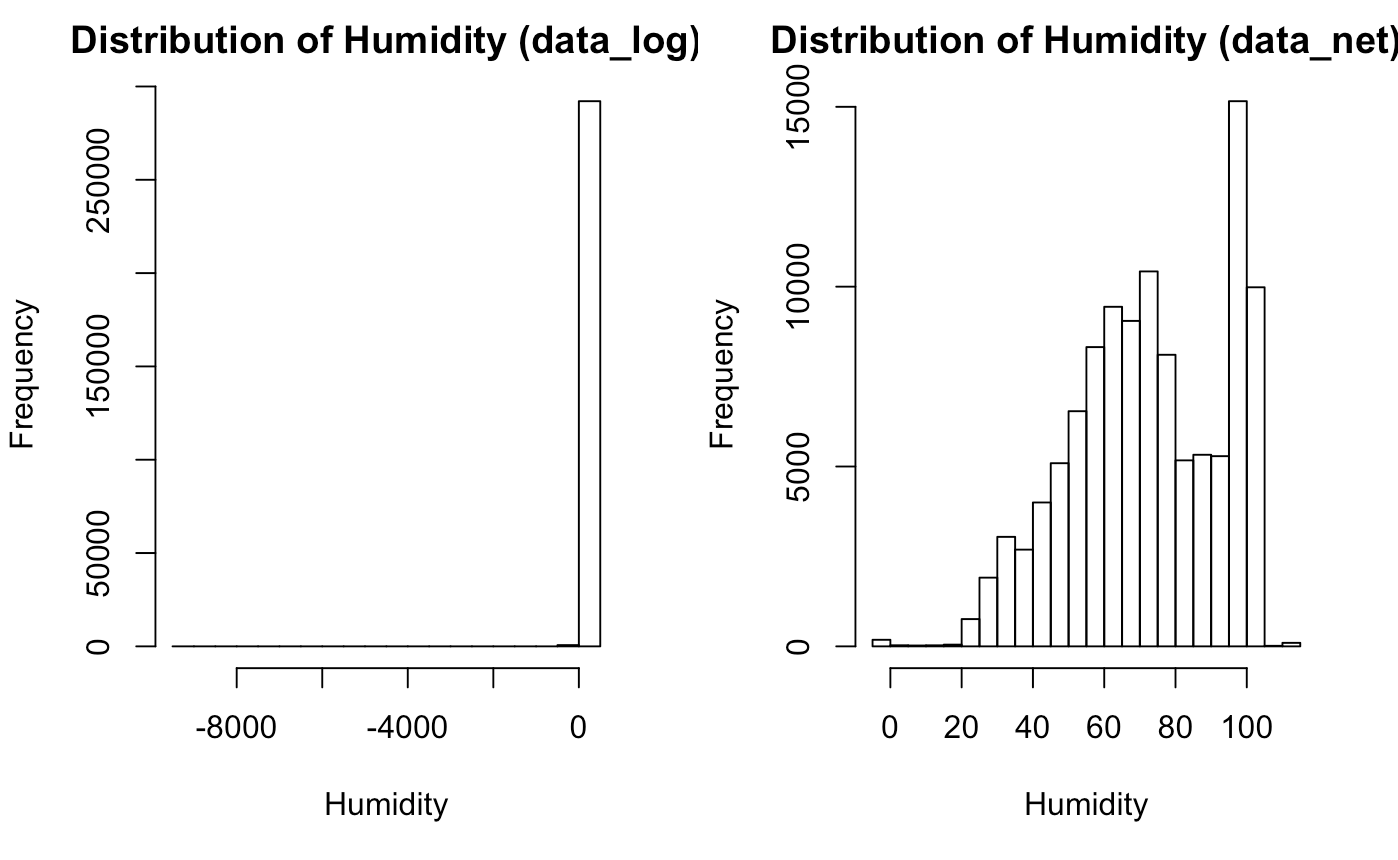
\includegraphics[width=85mm]{2a.png}
    \caption{}
    \label{fig:2a}
\end{figure}


The only variables that show a certain degree of consistency are  \textbf{hamatop}  and \textbf{hamabot}, which was later found out to be the two light levels: incidentPAR and reflectedPAR. For example, the distributions of incidentPAR are shown in Fig.2.:  

\begin{figure}
    \centering
    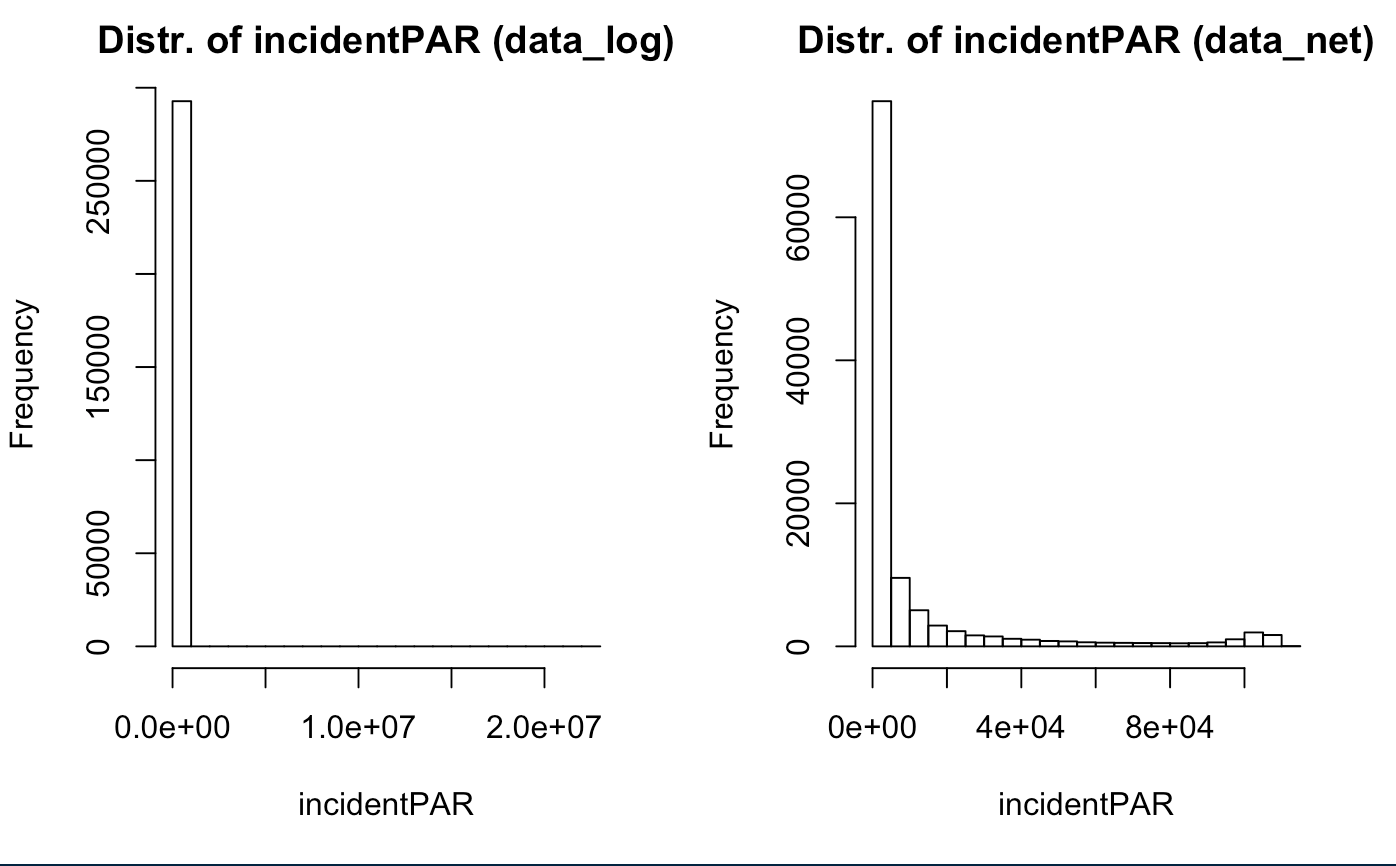
\includegraphics[width=85mm]{2a2.png} 
    \caption{}
    \label{fig:2a2}
\end{figure}



It was noticed that the incidentPAR and reflectedPAR values from both datasets have a very broad range, particularly incidentPAR: its values range from 0 to over 60000. We suspected that these values may have been recorded with lux rather than PPFD (the unit used in the paper). With such assumption and an attempt to convert data to the same range to reach consistency, we divided all values of incidentPAR and reflectedPAR by 54 to convert the unit from lux to PPFD. 

While viewing the summaries of each of the variables, we discovered that there is only one result time for all data points in data\_log. It is suspected that such time is the time at which the data was imported from the local machines to the network lab. This column is thus not useful for our purpose of tracking time and was therefore removed.
\subsection{Remove Missing Values}

The summaries of the variables also suggest that there are many missing values marked as NA in all datasets. Since the number of missing values does not take up a significant proportion of the total data and such missing values may bring in trouble and inconvenience later during data exploration, we have decided to remove them. There are in total \textbf{4262} missing values in \texttt{data\_net} and \textbf{8270} in \texttt{data\_log}, which take up to only about \textbf{3.7} percent and \textbf{7.1} percent of the total number of values in the \textbf{humidity} datasets.

To take a deeper look at the missing values, we found the corresponding dates (result\_time) of these NAs and created a plot of the missing measurements with their corresponding dates. The data is taken from the network dataset only as the time listed in log dataset are all the same and was deleted earlier. 

\begin{figure}
    \centering
    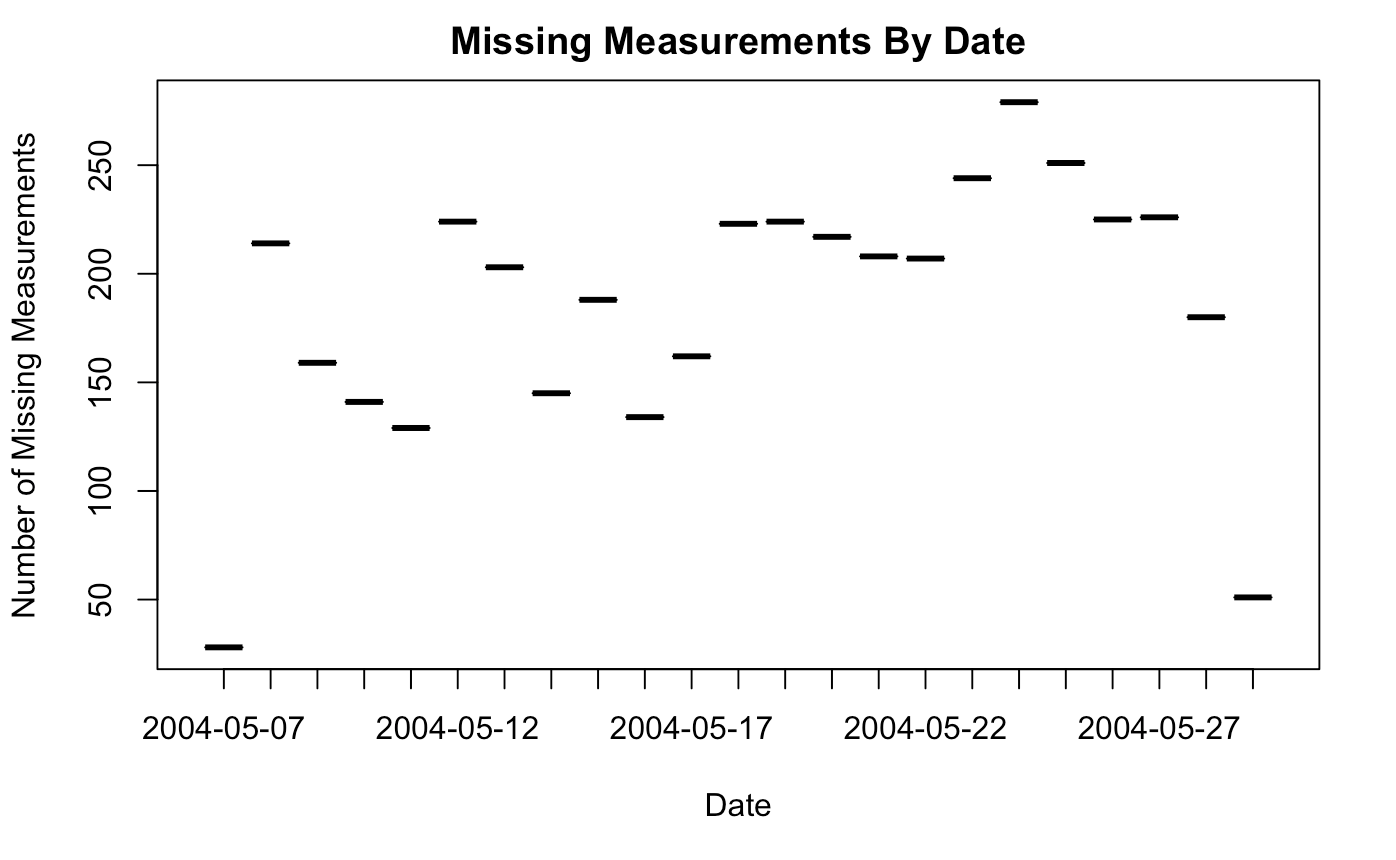
\includegraphics[width=85mm]{2b.png} 
    \caption{}
    \label{fig:2b}
\end{figure}
 

The graph Fig.3 indicates that the missing values were all in the dates between May 7th and May 27th. The number of missing values flutuate significantly throughout this 20-day period. One potential reason for such missing measurements is the instability of the battery or the sensors themselves throughout the time period.
\subsection{Remove Outliers}

The humidity is checked by reading through the summary of the data associated with this variable. Since humidity is recorded in relative terms (as a percentage), the value should approximately be in the range of 0 to 100. However, the summary indicates that the minimum humidity reading of the net data was as low as -9000 and the maximum reading for both net data and log data was above 100. The abnormal readings of humidity were probably due to problems with the sensors themselves since the ones associated with abnormal battery voltage were already removed. Since such readings are difficult to interpret, all data with humidity below 0 or above 100 were removed from the datasets.

A boxplot of the temperature for the merged dataset was created to check for outliers. 

\begin{figure}
    \centering
    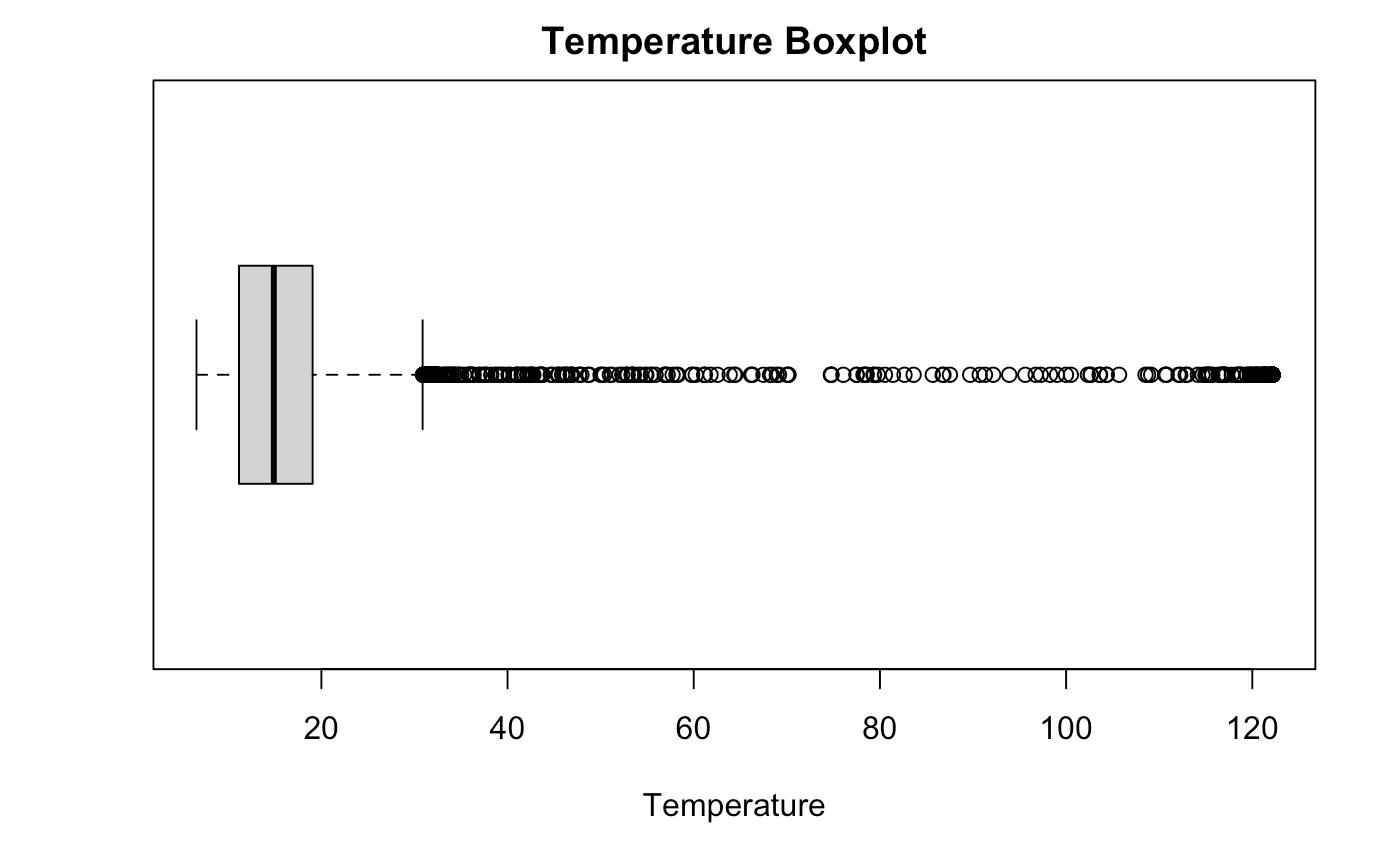
\includegraphics[width=85mm]{2d.png} 
    \caption{}
    \label{fig:2d}
\end{figure}


According to the boxplot Fig.4, the data points even further to the right of the whisker boundary are considered outliers. Such conjecture was confirmed by the quantile information of the data, which indicates that the 75 percentile temperature is 19.0574 but the 100 percentile temperature is 122.1530. Therefore, R was used to find the specific value (cutting line) for the whisker upper boundary and all values outside of this boundary were removed.

Having read through the description of the sensors in the research paper, we discovered that \textbf{hamatop} and \textbf{hamabot} represent the two light levels: incidentPAR and reflectedPAR. Having plotted their boxplots, we noticed that both plots are very similar in that they both have large numbers of data points with the value of zero. We decided not to remove these zero values as they took up a considerable proportion of the total data and these values may have been collected during night time when no sunlight was detected.

According to the research paper, many of the outliers appear to be collected when the battery voltage was at an abnormal range (when the batteries of the sensors did not work properly). Therefore, we applied the same method listed in the paper to remove the outliers: remove all data points from which the voltage is outside of the normal range (lower than 2.4 or greater than 3). Having observed the voltage values for both datasets, we found out that coltage in net data are all well outside of the normal range (min: 198), while most of the voltage values in the \texttt{data\_log} are within the normal range (2.4 to 3). We suspect that either the units are different or the voltage in \texttt{data\_net} is not a record of the battery voltage (e.g. the voltage output of the laboratory from which the network data is received). Since there is no strong evidence supporting either conjecture, this voltage data was left as it is at this stage.

A boxplot of the IDs of all the nodes was plotted to check if there is any abnormality. 

\begin{figure}
    \centering
    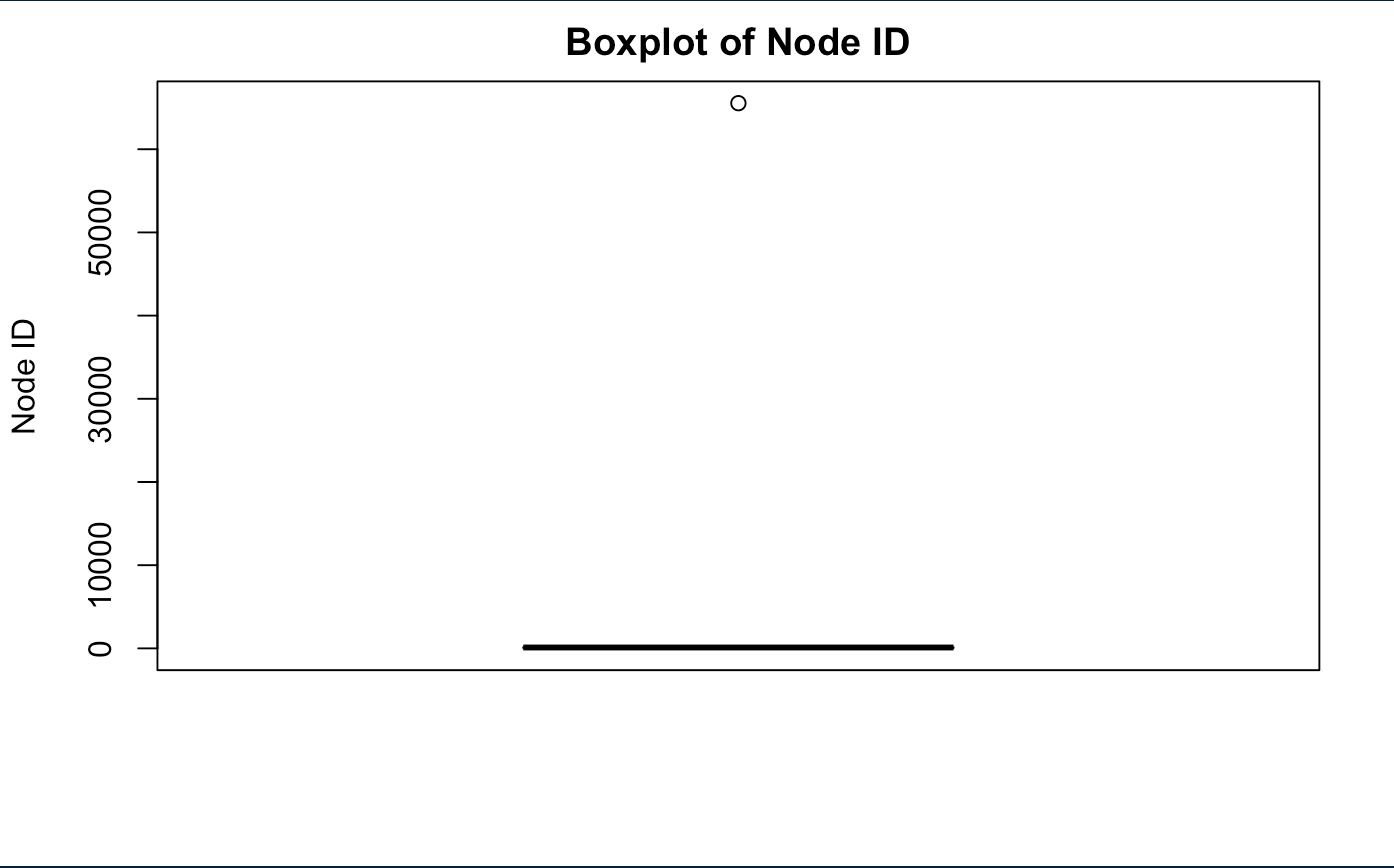
\includegraphics[width=85mm]{2e.png} 
    \caption{}
    \label{fig:2e}
\end{figure}


As shown by the boxplot Fig.5, the majority of the nodes have id values that are very small but there is one value well above the normal range. The quantile information of the nodeid further confirms the conjecture that there is one abnormal id whose value is unusually high: the 75 percentile value is 127, while the 100 percentile is 65535. Since this is clearly wrong and may affect later analysis, that node was removed from the dataset.

\subsection{Merge Datasets}

After data cleaning was implemented to both \texttt{data\_log} and \texttt{data\_net}, the two datasets were merged by matching each of their unique node IDs and epoch values, resulting in a merged dataset with 6 columns. This adds 5 additional columns to the main table, and increases the number of variables to 11.

\section{Data Exploration}
\subsection{Relationship Between Variables}

A scatterplot was created to examine the relationship between temperature and humidity in Fig.6.

\begin{figure}
    \centering
    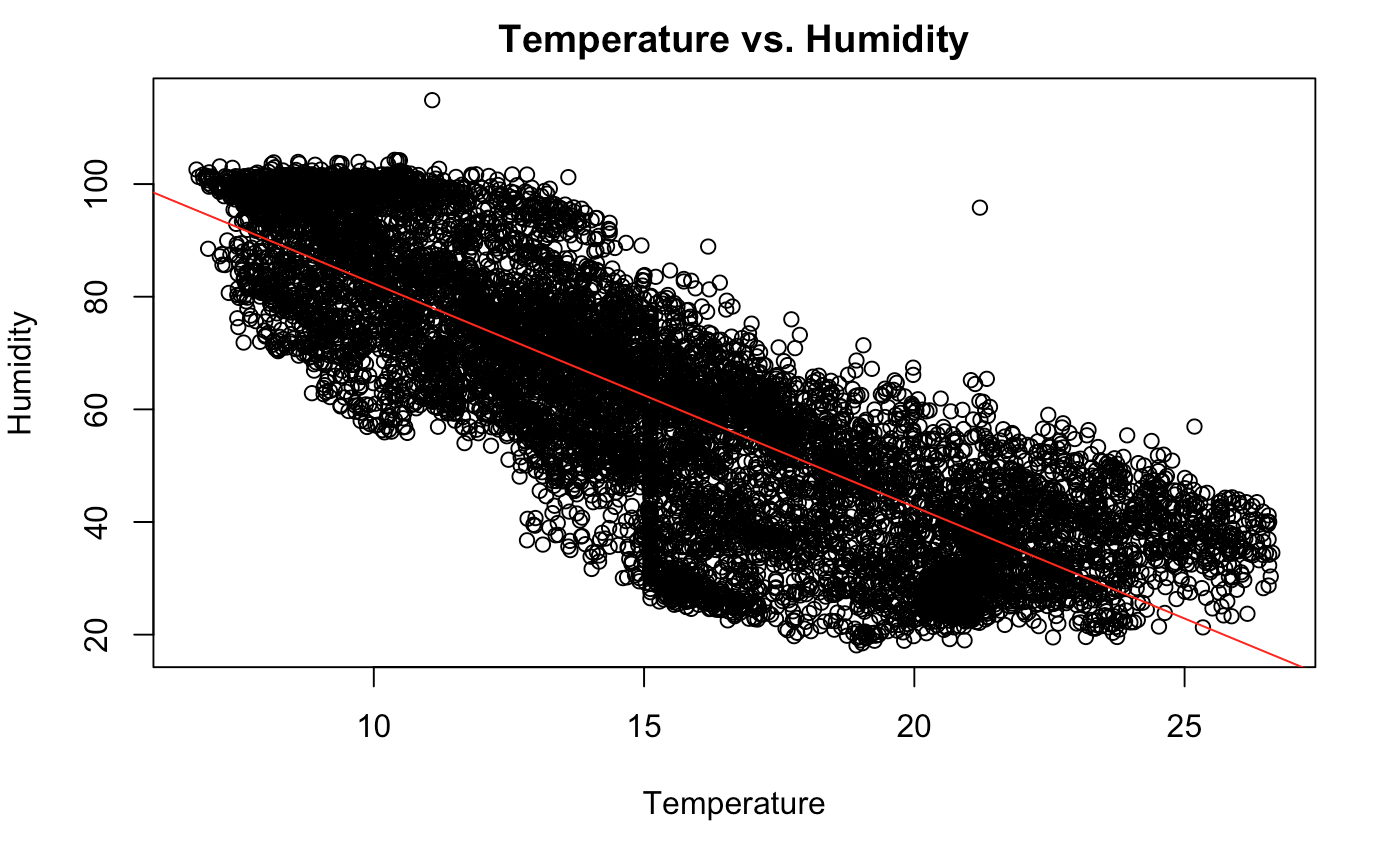
\includegraphics[width=85mm]{3a.png} 
    \caption{}
    \label{fig:3a}
\end{figure}

Instead of choosing a specific time interval, we used the entire dataset as we would like to observe the overall relationship between temperature and humidity throughout the experiment. However, only a random sample of 10000 data points were used to plot the graph as having all points in the graph makes it less visually appealing due to the abundance of overlapping points. Since the initial dataset is large enough, we believe that a random subset is sufficiently representative of the entire dataset.

Scatterplots were created for each variable against Incident PAR in Fig.8. The two variables that display the most distinct and interesting associations with Incident PAR are height and reflected PAR. 

\begin{figure}
    \centering
    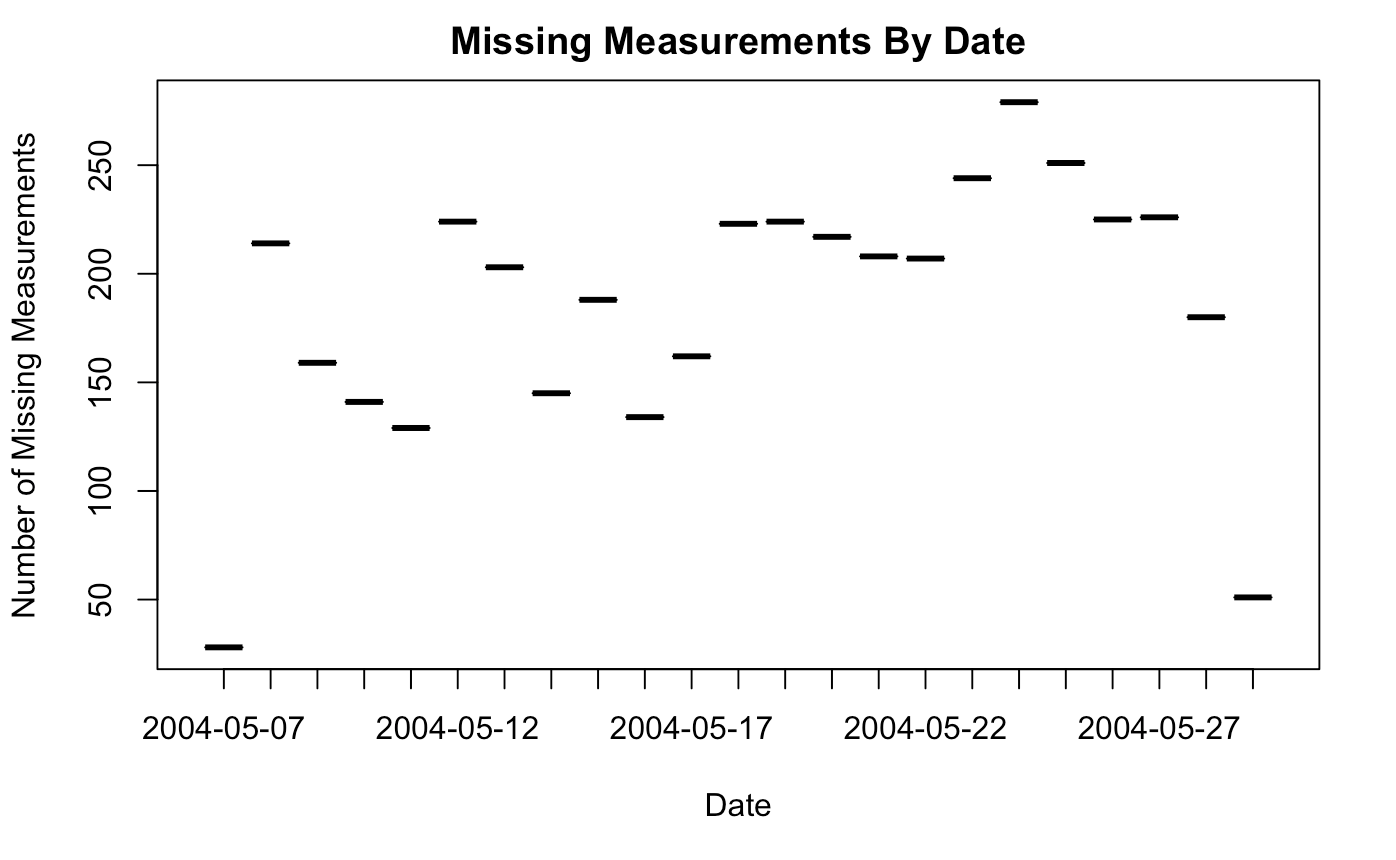
\includegraphics[width=85mm]{2b.png} 
    \caption{}
    \label{fig:2b}
\end{figure}

As shown by the graph Fig.8, as the height of the tree increases, the range of incident PAR increases, probably due to the fact that taller trees have greater exposure to sunlight. 

\begin{figure}
    \centering
    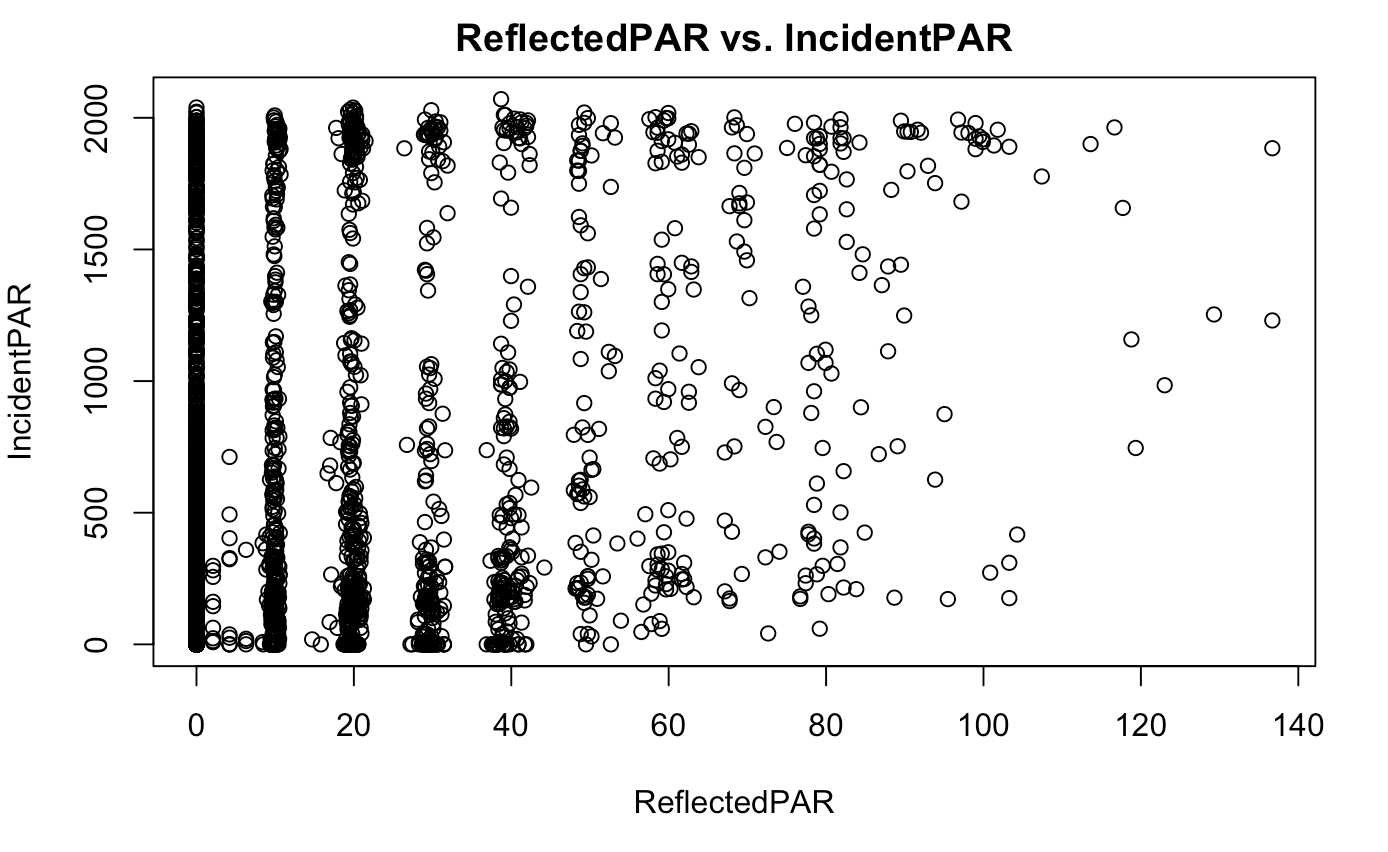
\includegraphics[width=85mm]{3b2.png} 
    \caption{}
    \label{fig:3b2}
\end{figure}

In addition, reflected PAR and incident PAR displays a unique bipolar trend: the points clustered around the minimum and maximum regions. When the value of reflected PAR is low, such as zero, the corresponding incident PAR values cover a wide range from its minimum to maximum value. However, as the reflected PAR value increases, the incident PAR value varies over a much smaller range. Such trend is obvious as by the time reflected PAR reaches 100, there are few corresponding incident PAR values present. 

\subsection{Time Series Analysis}

A time series analysis was conducted in which each of the major variables were plotted against time to observe the temporal trends, with height as color cue. Since height is a continuous variable and the dataset contains over 50 unique height values, a plot with each height representing a different color is visually difficult to interpret (because the high number of different colors interfere with each other in the graph). Therefore, we separated the heights into different groups with approximately equal number of nodes for each group. The time scale chosen is an entire day on May 1st instead a particular hour, the entire experiment, or any other random days. This is because according to the research paper, May 1st is the day that contains a wide variety of temperature and humidity values throughout the period and thus may reveal interesting patterns. Time was represented using the epoch variable. In all four graphs(Fig.9 to Fig.12), each curve represents a different sensor and each color corresponds to the heights of the sensors for which they were placed. 

\begin{figure}
    \centering
    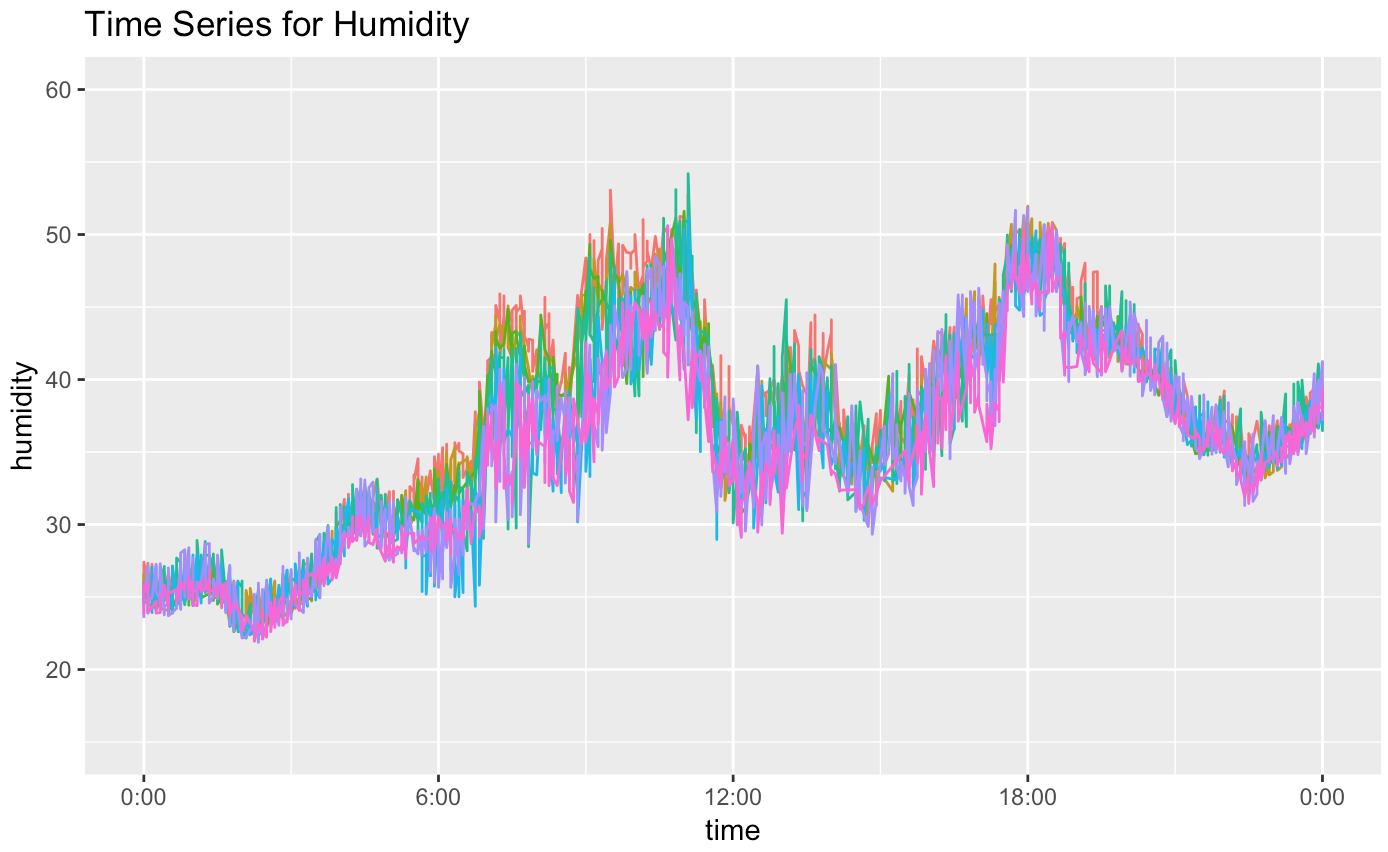
\includegraphics[width=85mm]{3c.png} 
    \caption{}
    \label{fig:3c}
\end{figure}

Since data cleaning was completed prior to plotting these graphs, the values for all variables fall into expected range. However, as shown by the graphs Fig.9, the values tend to concentrate in a smaller range comparing to the overall distribution. For example, although the overall humidity for the entire experiment ranges from around 15 to 80, the humidity values on May 1st are concentrated between 22 and 55. The plot indicates that humidity flutuates throughout the day and is at its peak by around noon time. The value is the lowest at the beginning and end of the day. In addition, sensors at all heights seem to follow approximately the same trend. 

\begin{figure}
    \centering
    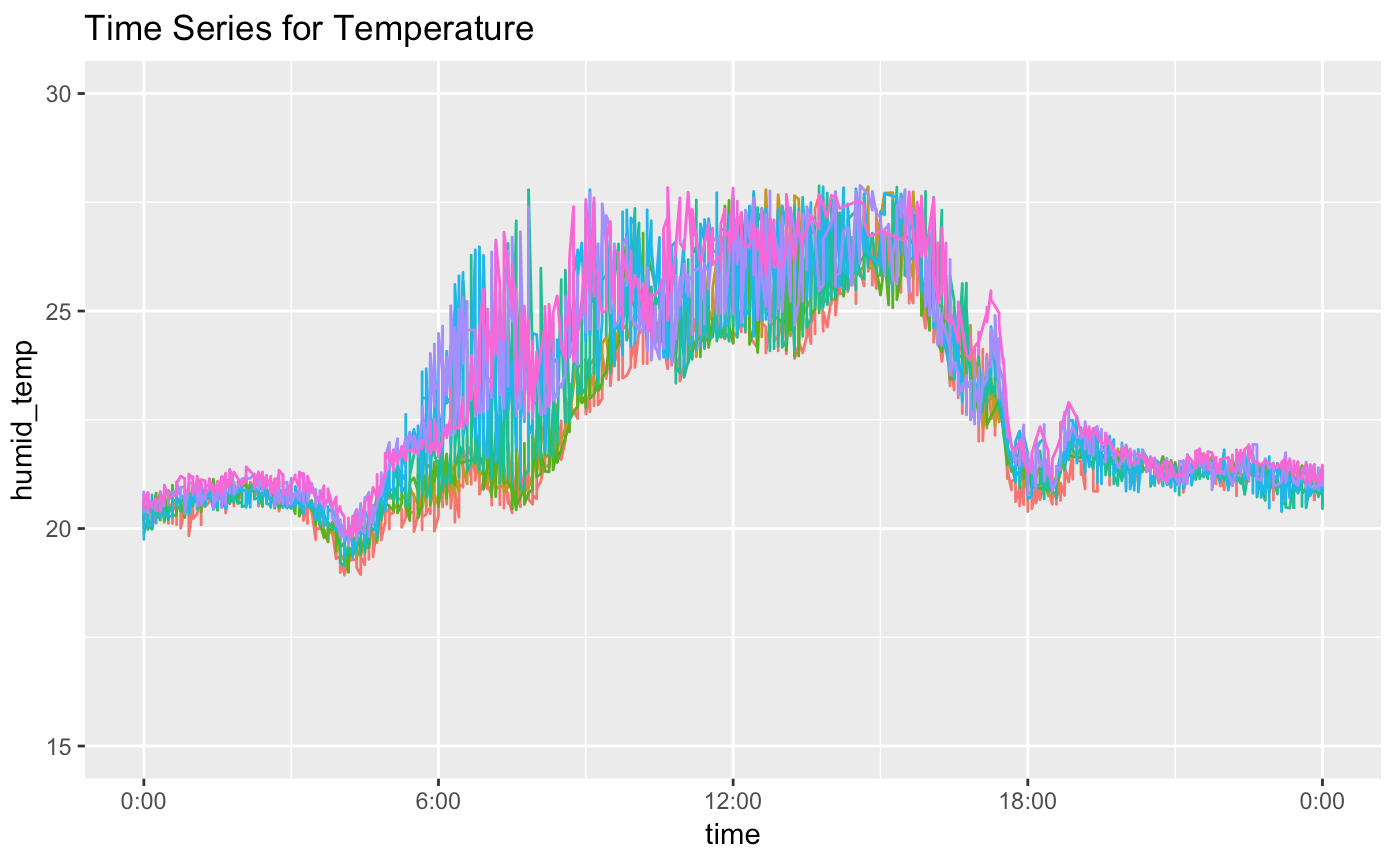
\includegraphics[width=85mm]{3c2.png} 
    \caption{}
    \label{fig:3c2}
\end{figure}


The plot for temperature against time shows a similar trend comparing to humidity, with the lowest values at the start and end of the day. However, comparing to the previous graph, nodes at different heights seem to behave inconsistently. This may be because nodes at a higher height will experience more exposure to sunlight and thus will have higher temperature. 

\begin{figure}
    \centering
    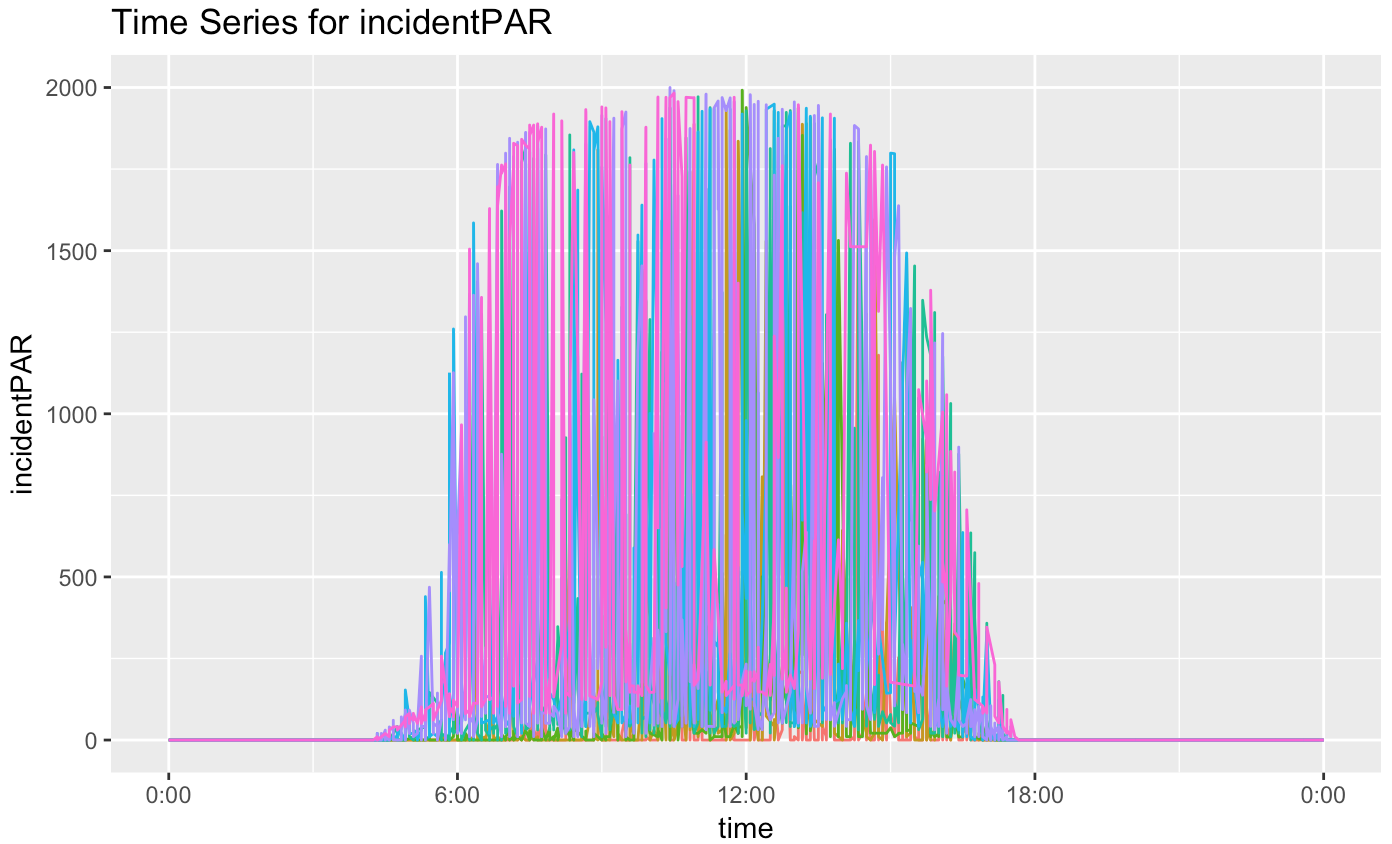
\includegraphics[width=85mm]{3c3.png} 
    \caption{}
    \label{fig:3c3}
\end{figure}


The time series plot for incident PAR against time indicates a strong pattern. At the start of the day, the values are zero but they increase drastically at around 5AM in the morning and falls quickly back to zero at almost 6PM. This is because the sunrise that cause sensors to receive more lights. The graph Fig.11 shows that the incident PAR values are relatively high and stable during the day and fall to zero around 6pm, it supports the conjecture made earlier in the data cleaning section, in which the abundance of zero values may be due to the fact that the sensors do not have light receptions at night. 

\begin{figure}
    \centering
    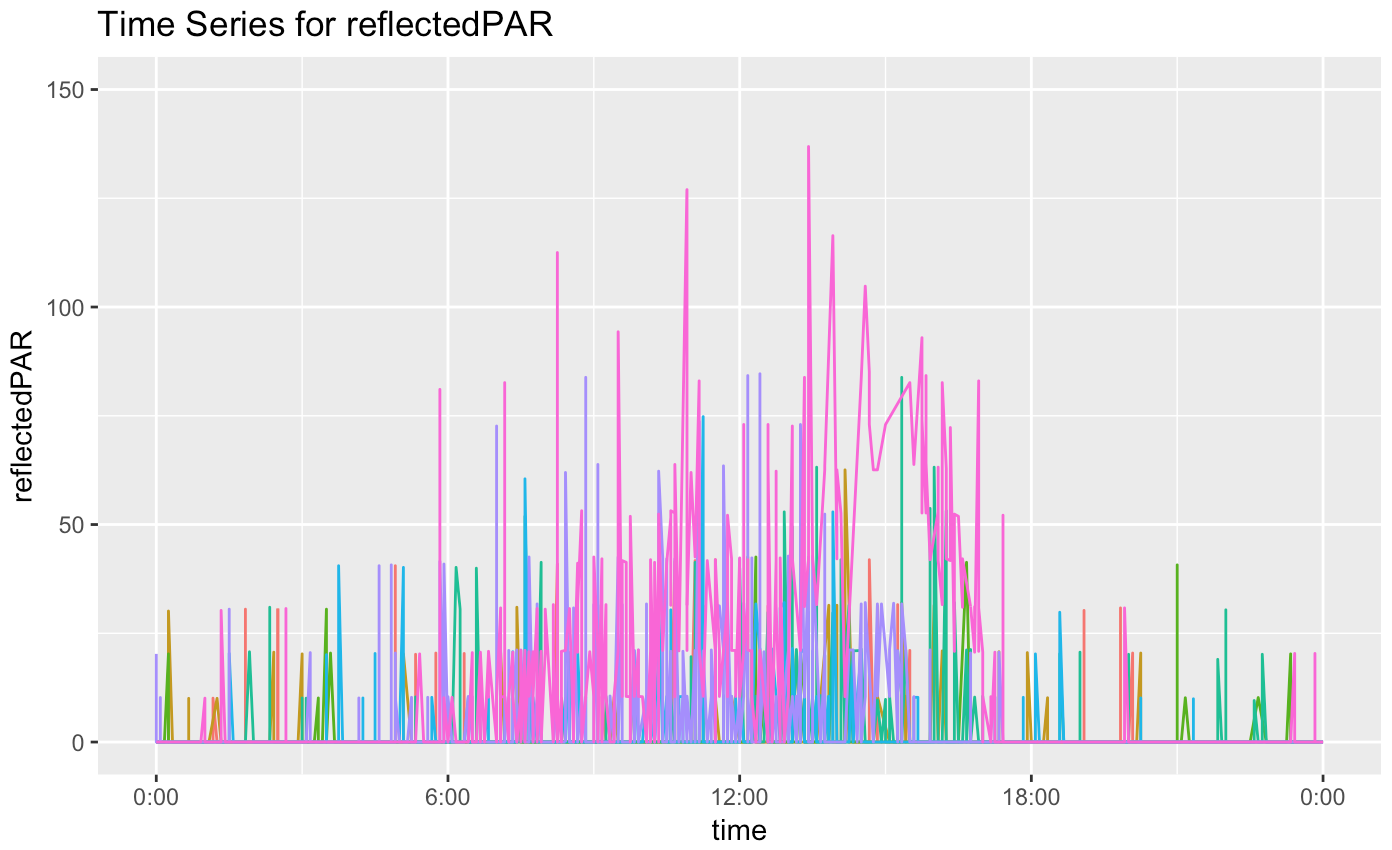
\includegraphics[width=85mm]{3c4.png} 
    \caption{}
    \label{fig:3c4}
\end{figure}


Similar to incident PAR, the plot for reflected PAR also shows relatively higher values in the middle of the day. However, the reflected PAR readings are relatively smaller, which are in the range of 0 to 150, comparing to incident PAR. This is because reflected PAR are received by the lights that went through forest canopy and then reflected by the ground, causing reflected PAR readings to be significantly smaller than incident PAR, whose value indicates the direct light.

\subsection{Principal Component Analysis}

The dataset used to to carry out principal component analysis had its Node ID column removed. This is because we believed that such data is categorical but PCA will only work on numerical data.

A screeplot was created to observe the significance of different principal components. 

\begin{figure}
    \centering
    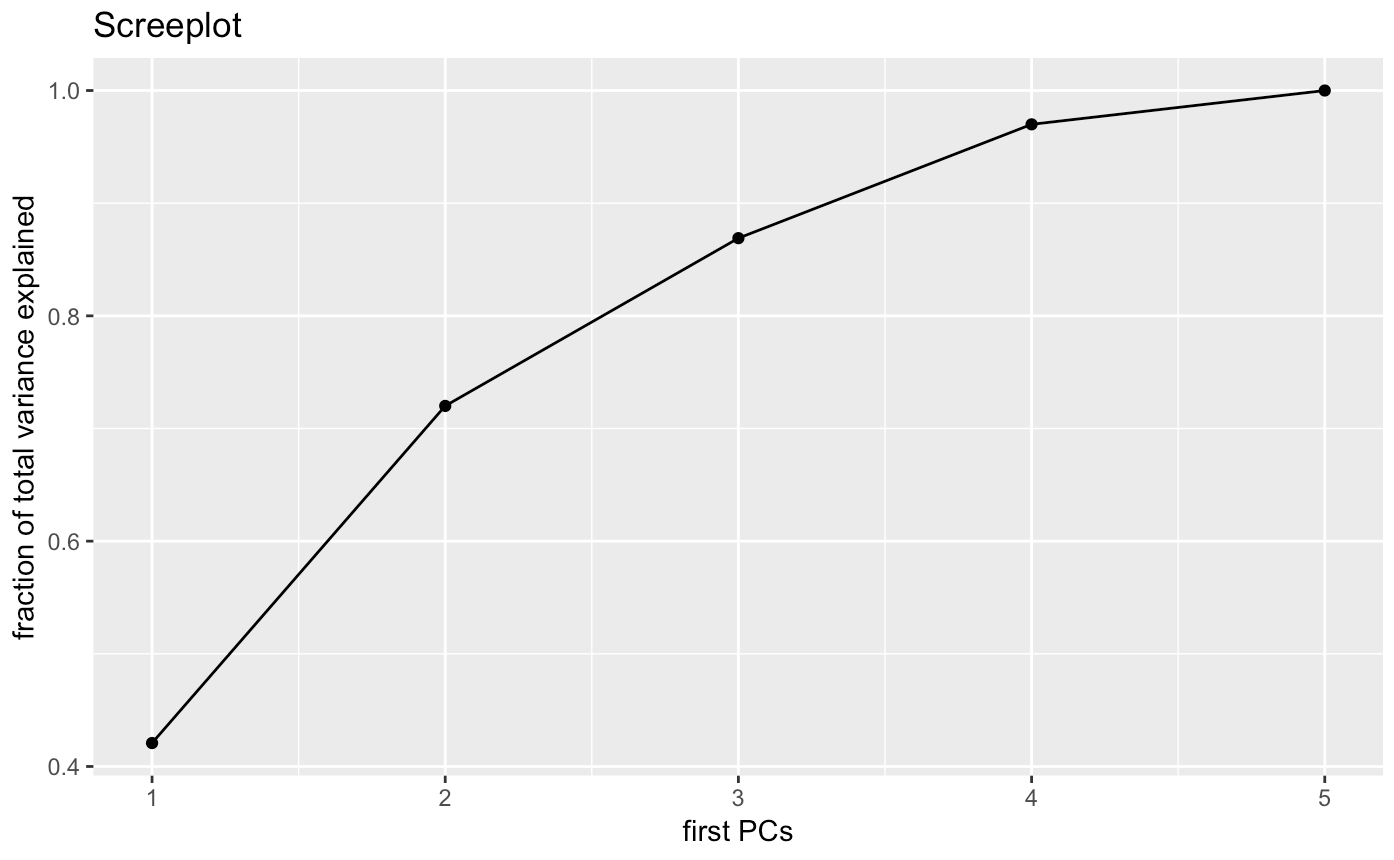
\includegraphics[width=85mm]{3d.png} 
    \caption{}
    \label{fig:3d}
\end{figure}


As shown in the graph Fig.13, the amount of variance captured by the PCs increase significantly between the first 3 PCs. The first 3 PCs captured up to 90 percent of the total variance and 4 PCs captured up almost 100 percent. This suggests that instead of having as many variables, the data could be approximated by a lower-dimension representation: 4 PCs or even 3 PCs may be sufficient. 

\section{Interesting Findings}

A scatterplot of temperature vs. height was made to observe the relationship between the two variables. Since we desired for a general trend between the variables, we took the average of each reading over 2000 epoch for each node. The value of 2000 was chosen as many of the nodes died after this time.

\begin{figure}
    \centering
    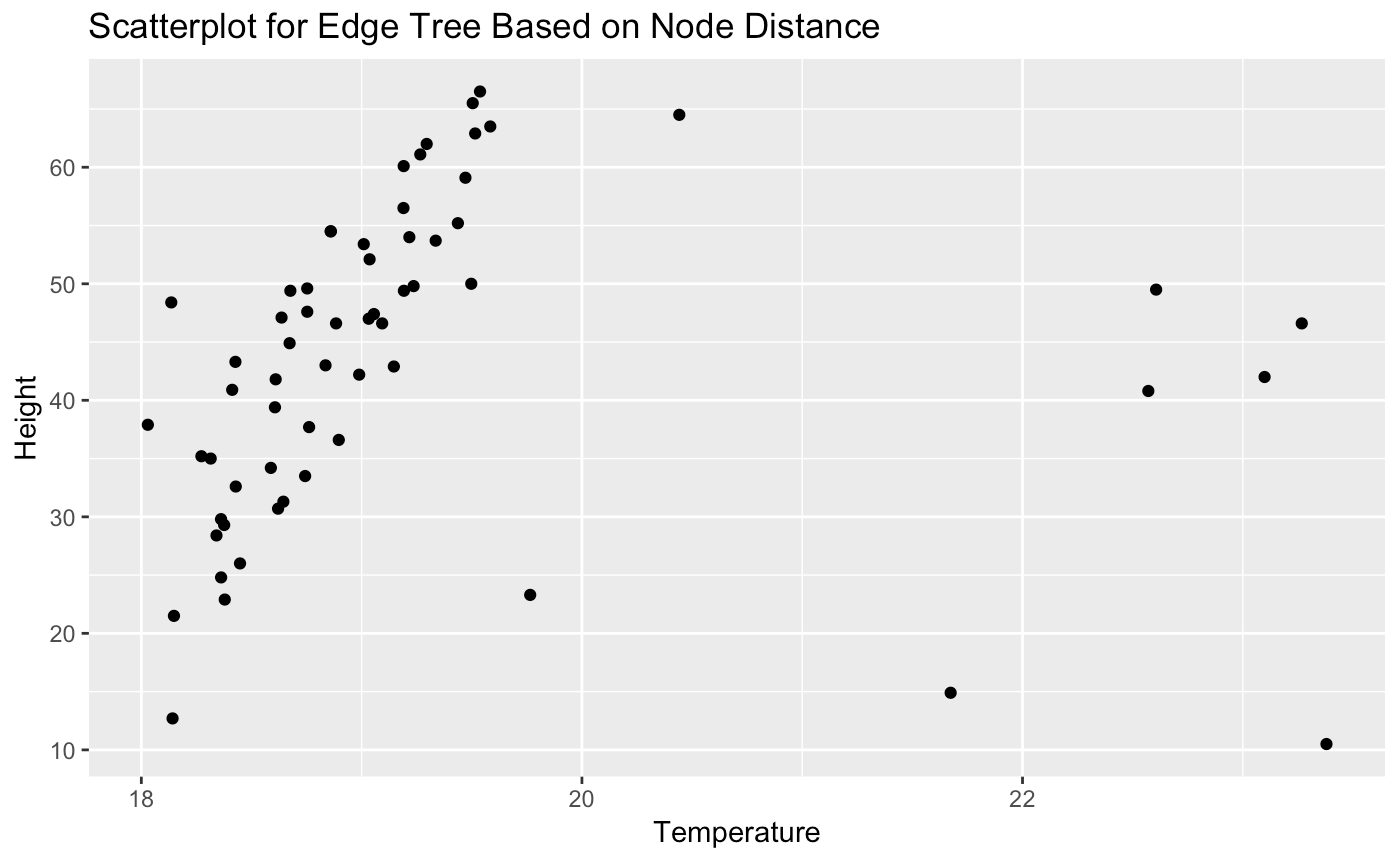
\includegraphics[width=85mm]{4a.png} 
    \caption{}
    \label{fig:4a}
\end{figure}

As shown by the plot Fig.14, although there are a few points of outliers, the overall patterns displayed is clear: temperature increases with rising height of the node. This may be because the higher the node is located, the more sunlight it is exposed to, thus leading to higher temperature. In addition, interior trees are in the center of the system and are more representative of the influence of the surrounding microclimate.  

Differences in humidity and temperature for trees at different locations were examined by comparing two boxplots. 

\begin{figure}
    \centering
    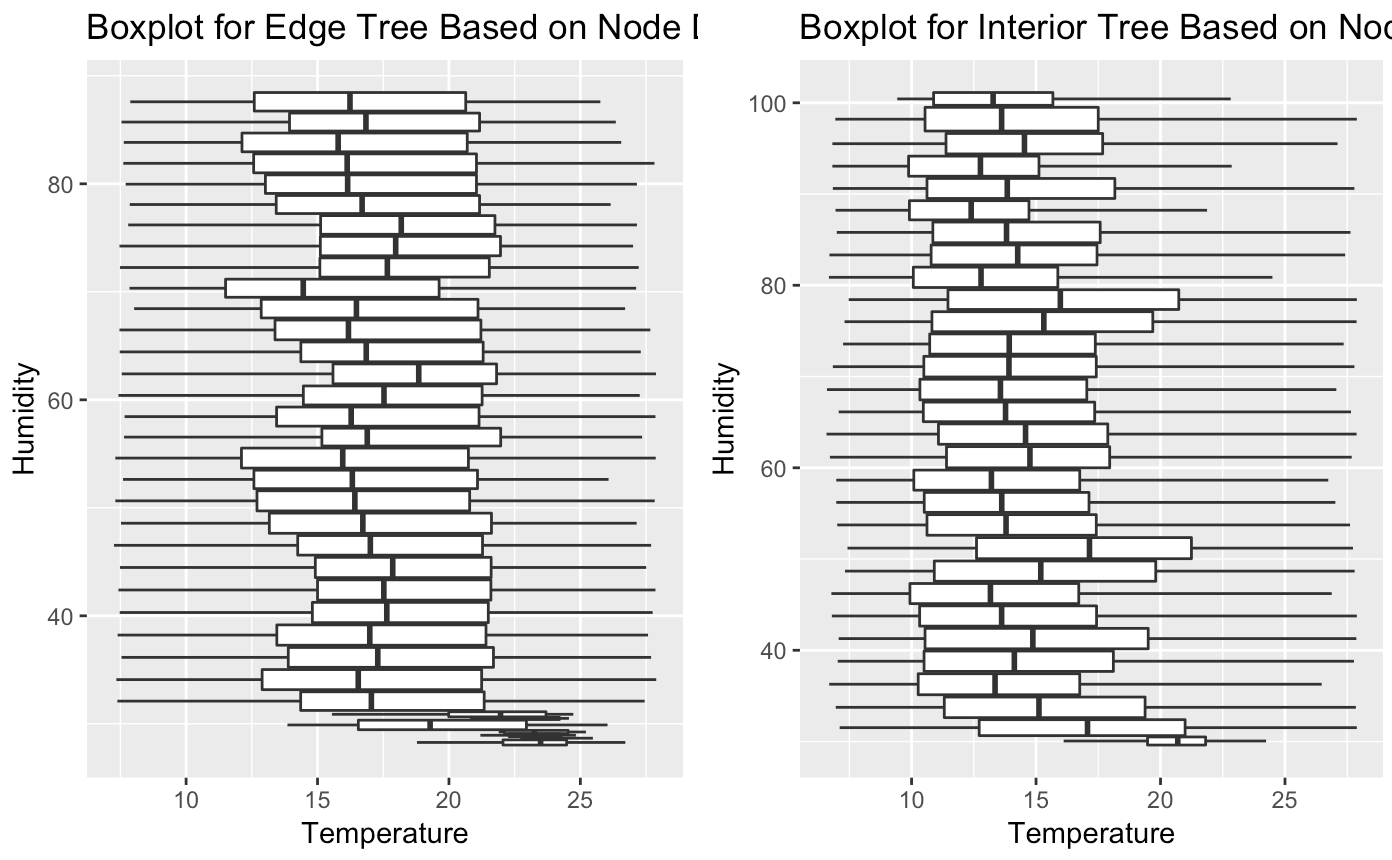
\includegraphics[width=85mm]{4b.png} 
    \caption{}
    \label{fig:4b}
\end{figure}

As shown by the two boxplots Fig.15, the edge trees tend to have on average a higher temperature of around 15, while the interior trees' temperatures are mostly slightly lower, at around 10. This is a reasonable trend as the interior trees tend to experience less exposure to sunlight and thus will have a relatively cooler temperature. Such lack of direct exposure to sunlight may also explain the fact that the interior trees' max humidity is also relatively higher. 

Another interesting finding was observed by the plot of height vs. mean humidity measured at the corresponding heightbased on different tree locations. 

\begin{figure}
    \centering
    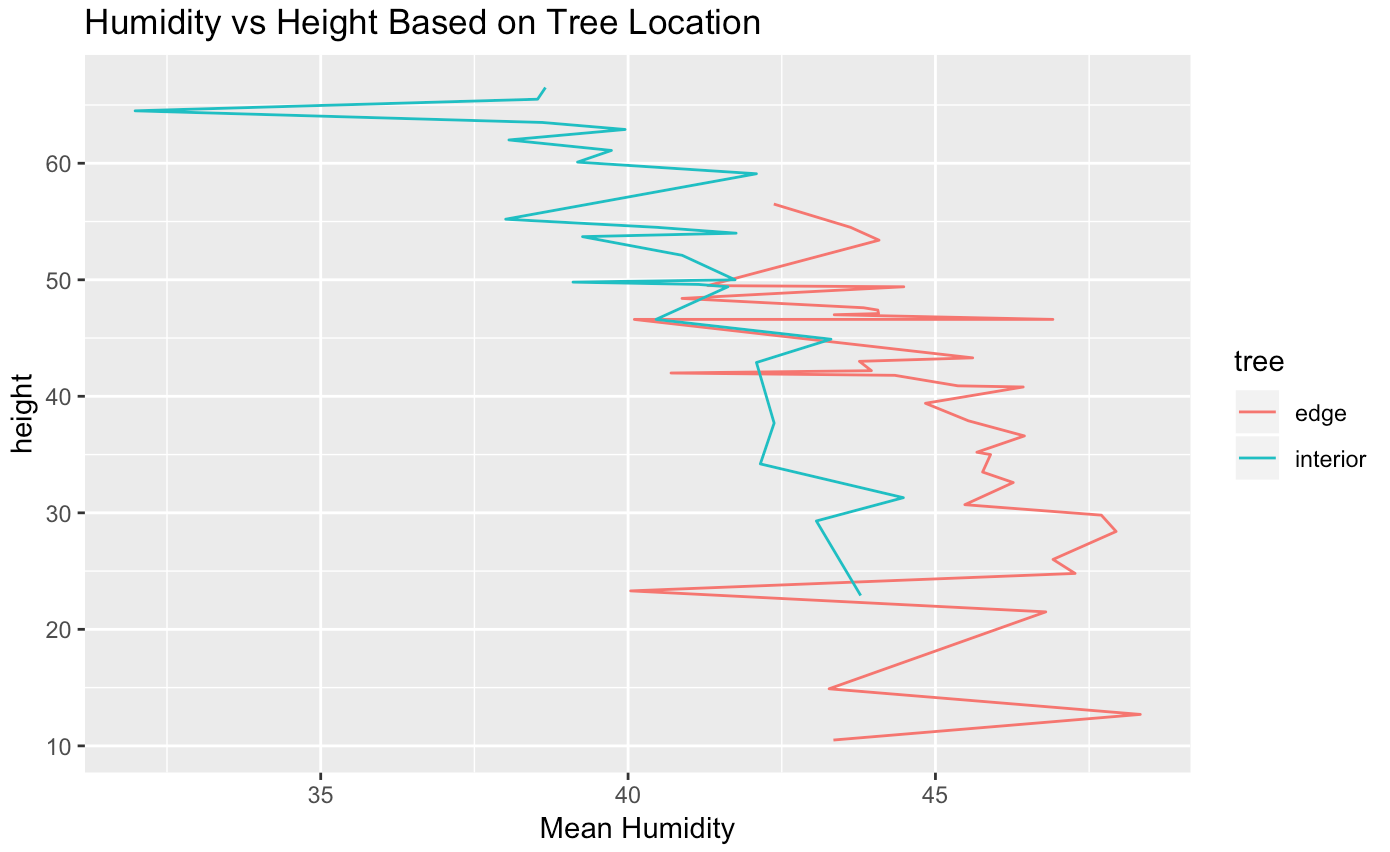
\includegraphics[width=85mm]{4c.png} 
    \caption{height vs. mean humidity}
    \label{fig:4c}
\end{figure}

Each of the lines represent the location of the tree. It is clear from the graph (Fig.16) that in most of the cases, at the same height, the interior trees' nodes will receive a higher humidity reading comparing to the edge tree nodes. 

\section{Graph Critique}
\subsection{Improvement of Sensor Reading Plots in 3a)}

Since both the plots of Incident PAR and Reflected PAR have long tails, they are highly skewed and can be difficult to interpret. A log transformation of the graphs is in this case appropriate since in R, log will automatically remove all values that were originally zero. Since the original histograms displayed in the research paper indicates that it is the zero value that has the highest frequency and leads to the long tails. Since we want to see the distributions among large values, we take the log transform of the original data points. The improved histograms are shown in Fig.17 and Fig.18. 

\begin{figure}
    \centering
    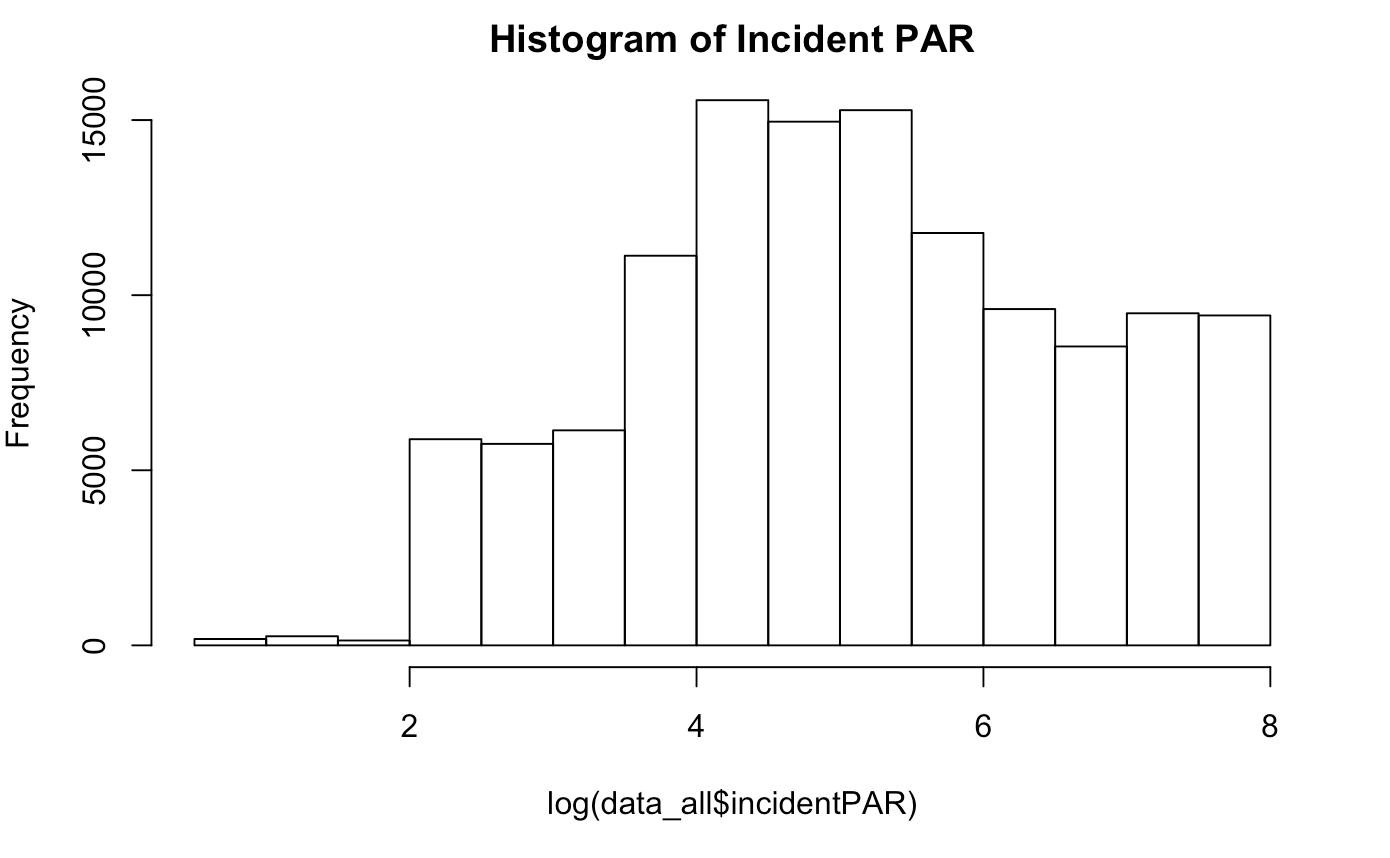
\includegraphics[width=85mm]{5a.png} 
    \caption{}
    \label{fig:5a}
\end{figure}

\begin{figure}
    \centering
    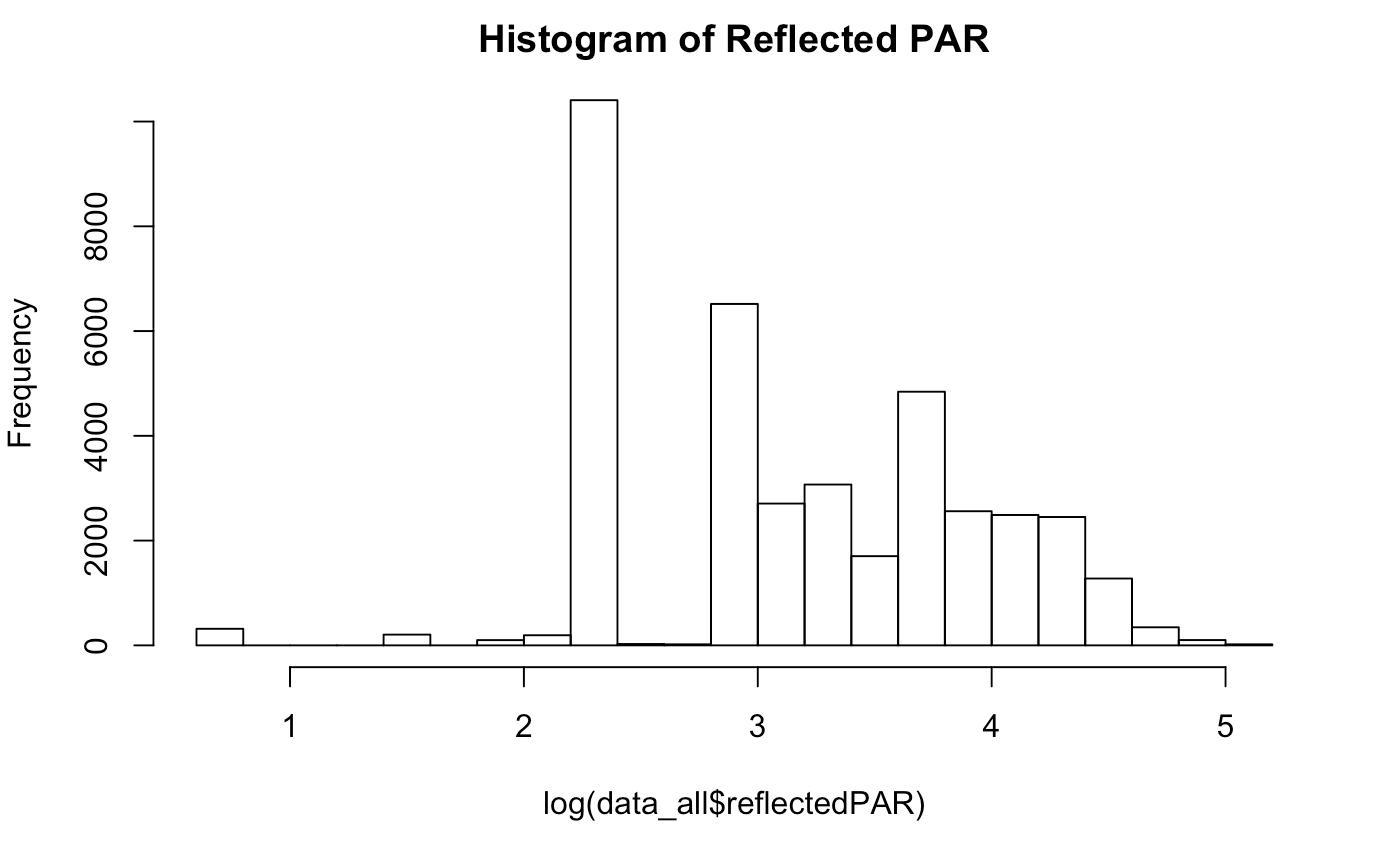
\includegraphics[width=85mm]{5a2.png} 
    \caption{}
    \label{fig:5a2}
\end{figure}

\subsection{Analysis of Plots in 3c) and 3d)}

In the original research paper, Boxplot 3c) displays the distribution of all the readings taken by the sensors at each height. Boxplot 3c) and Boxplot 3d)shows the distribution of the differeces between each sensor reading at each timestep and the mean of all the sensor readings. Though the graphs in figure 3 shows that there exists a trend in which the higher the height of node in the tree, the less likely that it is covered by the leaves and the higher chance of receiving a higher PAR, one major issue with these graphs is that they have neglected the role that time plays in this role: the graphs in Boxplot 3c) and Boxplot 3d) only takes into account the entire data set throughtout the experiment, thus they might not reflect the trend that we are interested. Since we are more interested in the variations within a short time period not the whole process.

To take the time factor into consideration, we specifically chose data from the timestep: 1062, representing 9:35 AM of May 1st, and created a scatterplot for this. 

\begin{figure}
    \centering
    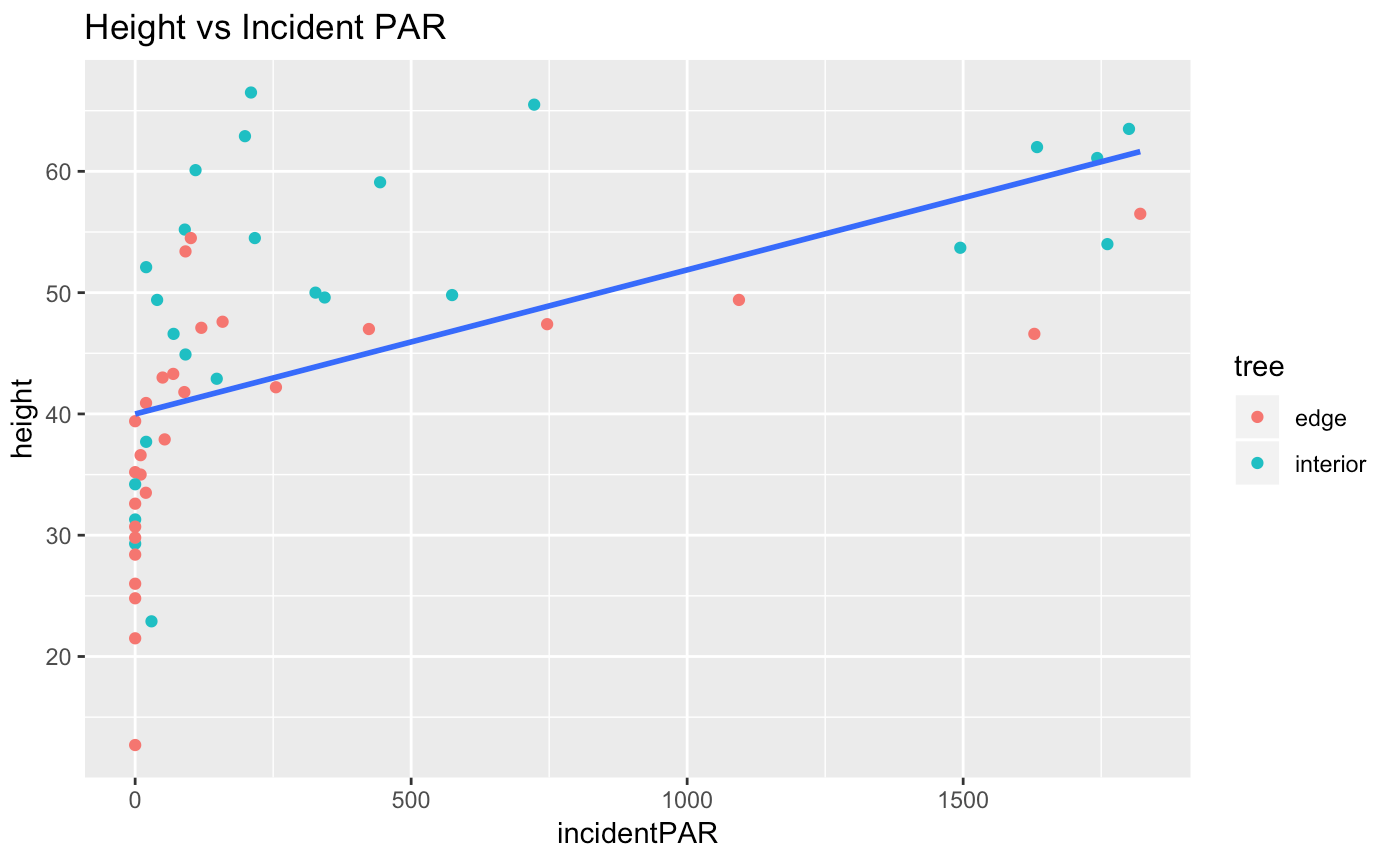
\includegraphics[width=85mm]{5b.png} 
    \caption{}
    \label{fig:5b}
\end{figure}

The plot indicates the same trend as the one implied by the graphs Figure 4 in the original research paper: the higher the height of the node, the higher the value of the Incident PAR. However, the claim is in a way stronger in that we have confirmed that having taken into the consideration of time, the pattern is still the same. 

\subsection{Suggestions For Improvement of Figure 4}

In Figure 4 of the research paper, it was very difficult to distinguish the colors of the lines in the two plots as some colors appear multiple times and this may cause confusion for readers without a clear legend displayed. Therefore, the variables may be organized into different groups before plotted, so that there are less lines with distinct colors and may potentially make the pattern easier to examine. However, grouping lines are challenging In addition, different grouping methods and needs lead to different grouping. Furthermore, after carefully examine the original graphs in Figure 4, we believe that each lines are represented by different node. A suggestion to the original Figure 4 is that a detailed legend would be useful in helping the reader to differentiate the lines, or reduce the number of lines by choosing a good grouping method.

\subsection{Analysis of Figure 7}

The plots in Figure 7 shows a direct contrast between the data stored in the local log and the data received over the network. The second plot under 7b) indicates that by Day 26, most of the nodes may have died out due to dying batteries and so the information obtained dropped significantly. Another interesting phenomenon is that in the fourth graph under Figure 7a), there appears to be a period in which no data was recorded at all. This may have been due to the failure of the network to deliver the data, though the sensors worked properly at the time because the corresponding graph of the local log suggests that there is no large chunk of missing data. 

Another way to visualize the difference between network data and local log data is to plot the distributions of the major variables from both datasets and compare them side by side. If the two datasets are similar, then the distributions should also be similar. However, since there are many disparities between the data from network and the data stored in the local log, one shall see completely different distributions for each variable. 

% %%%%%%%%%%%%%%%%%%%%%%%%%%%%%%%%%%%%%%%%%%%%%%%%%%%%%%%%%%%%%%%%%%%%%%
% \section{Footnotes\protect\footnotemark}
% \footnotetext{Examine the input file, asme2ej.tex, to see how a footnote is given in a head.}

% Footnotes are referenced with superscript numerals and are numbered consecutively from 1 to the end of the paper\footnote{Avoid footnotes if at all possible.}. Footnotes should appear at the bottom of the column in which they are referenced.

\section{References}

[1]Tolle, Gilman, et al. “A Macroscope in the Redwoods.” Proceedings of the 3rd International Conference on Embedded Networked Sensor Systems - SenSys 05, 2005, doi:10.1145/1098918.1098925.

[2] “Conversion - PPFD to Lux.” Apogee Instruments, Inc., www.apogeeinstruments.com/conversion-ppfd-to-lux/.

[3] Majasalmi, Titta. (2015). Estimation of leaf area index and the fraction of absorbed photosynthetically active radiation in a boreal forest. Dissertationes Forestales. 10.14214/df.187.

\end{document}
